\documentclass[11pt]{homework}

\newcommand{\hwname}{Minreng Wu}
\newcommand{\hwuin}{529005234 }
% \newcommand{\hwmajor}{CEEN}
\newcommand{\hwtype}{Project}
\newcommand{\hwnum}{\#1}
\newcommand{\hwclass}{CSCE-608}
\newcommand{\hwlecture}{}
\newcommand{\hwsection}{}

% This is just used to generate filler content. You don't need it in an actual
% homework!
\usepackage{lipsum}

\begin{document}
\maketitle

% Part 1
\question*{Application Description}

Technical blog is a very popular way for software engineers to share personal development experience 
with the other developers and learn new techniques. Below is the blog site called DZone which I visited
most:

\begin{center}
  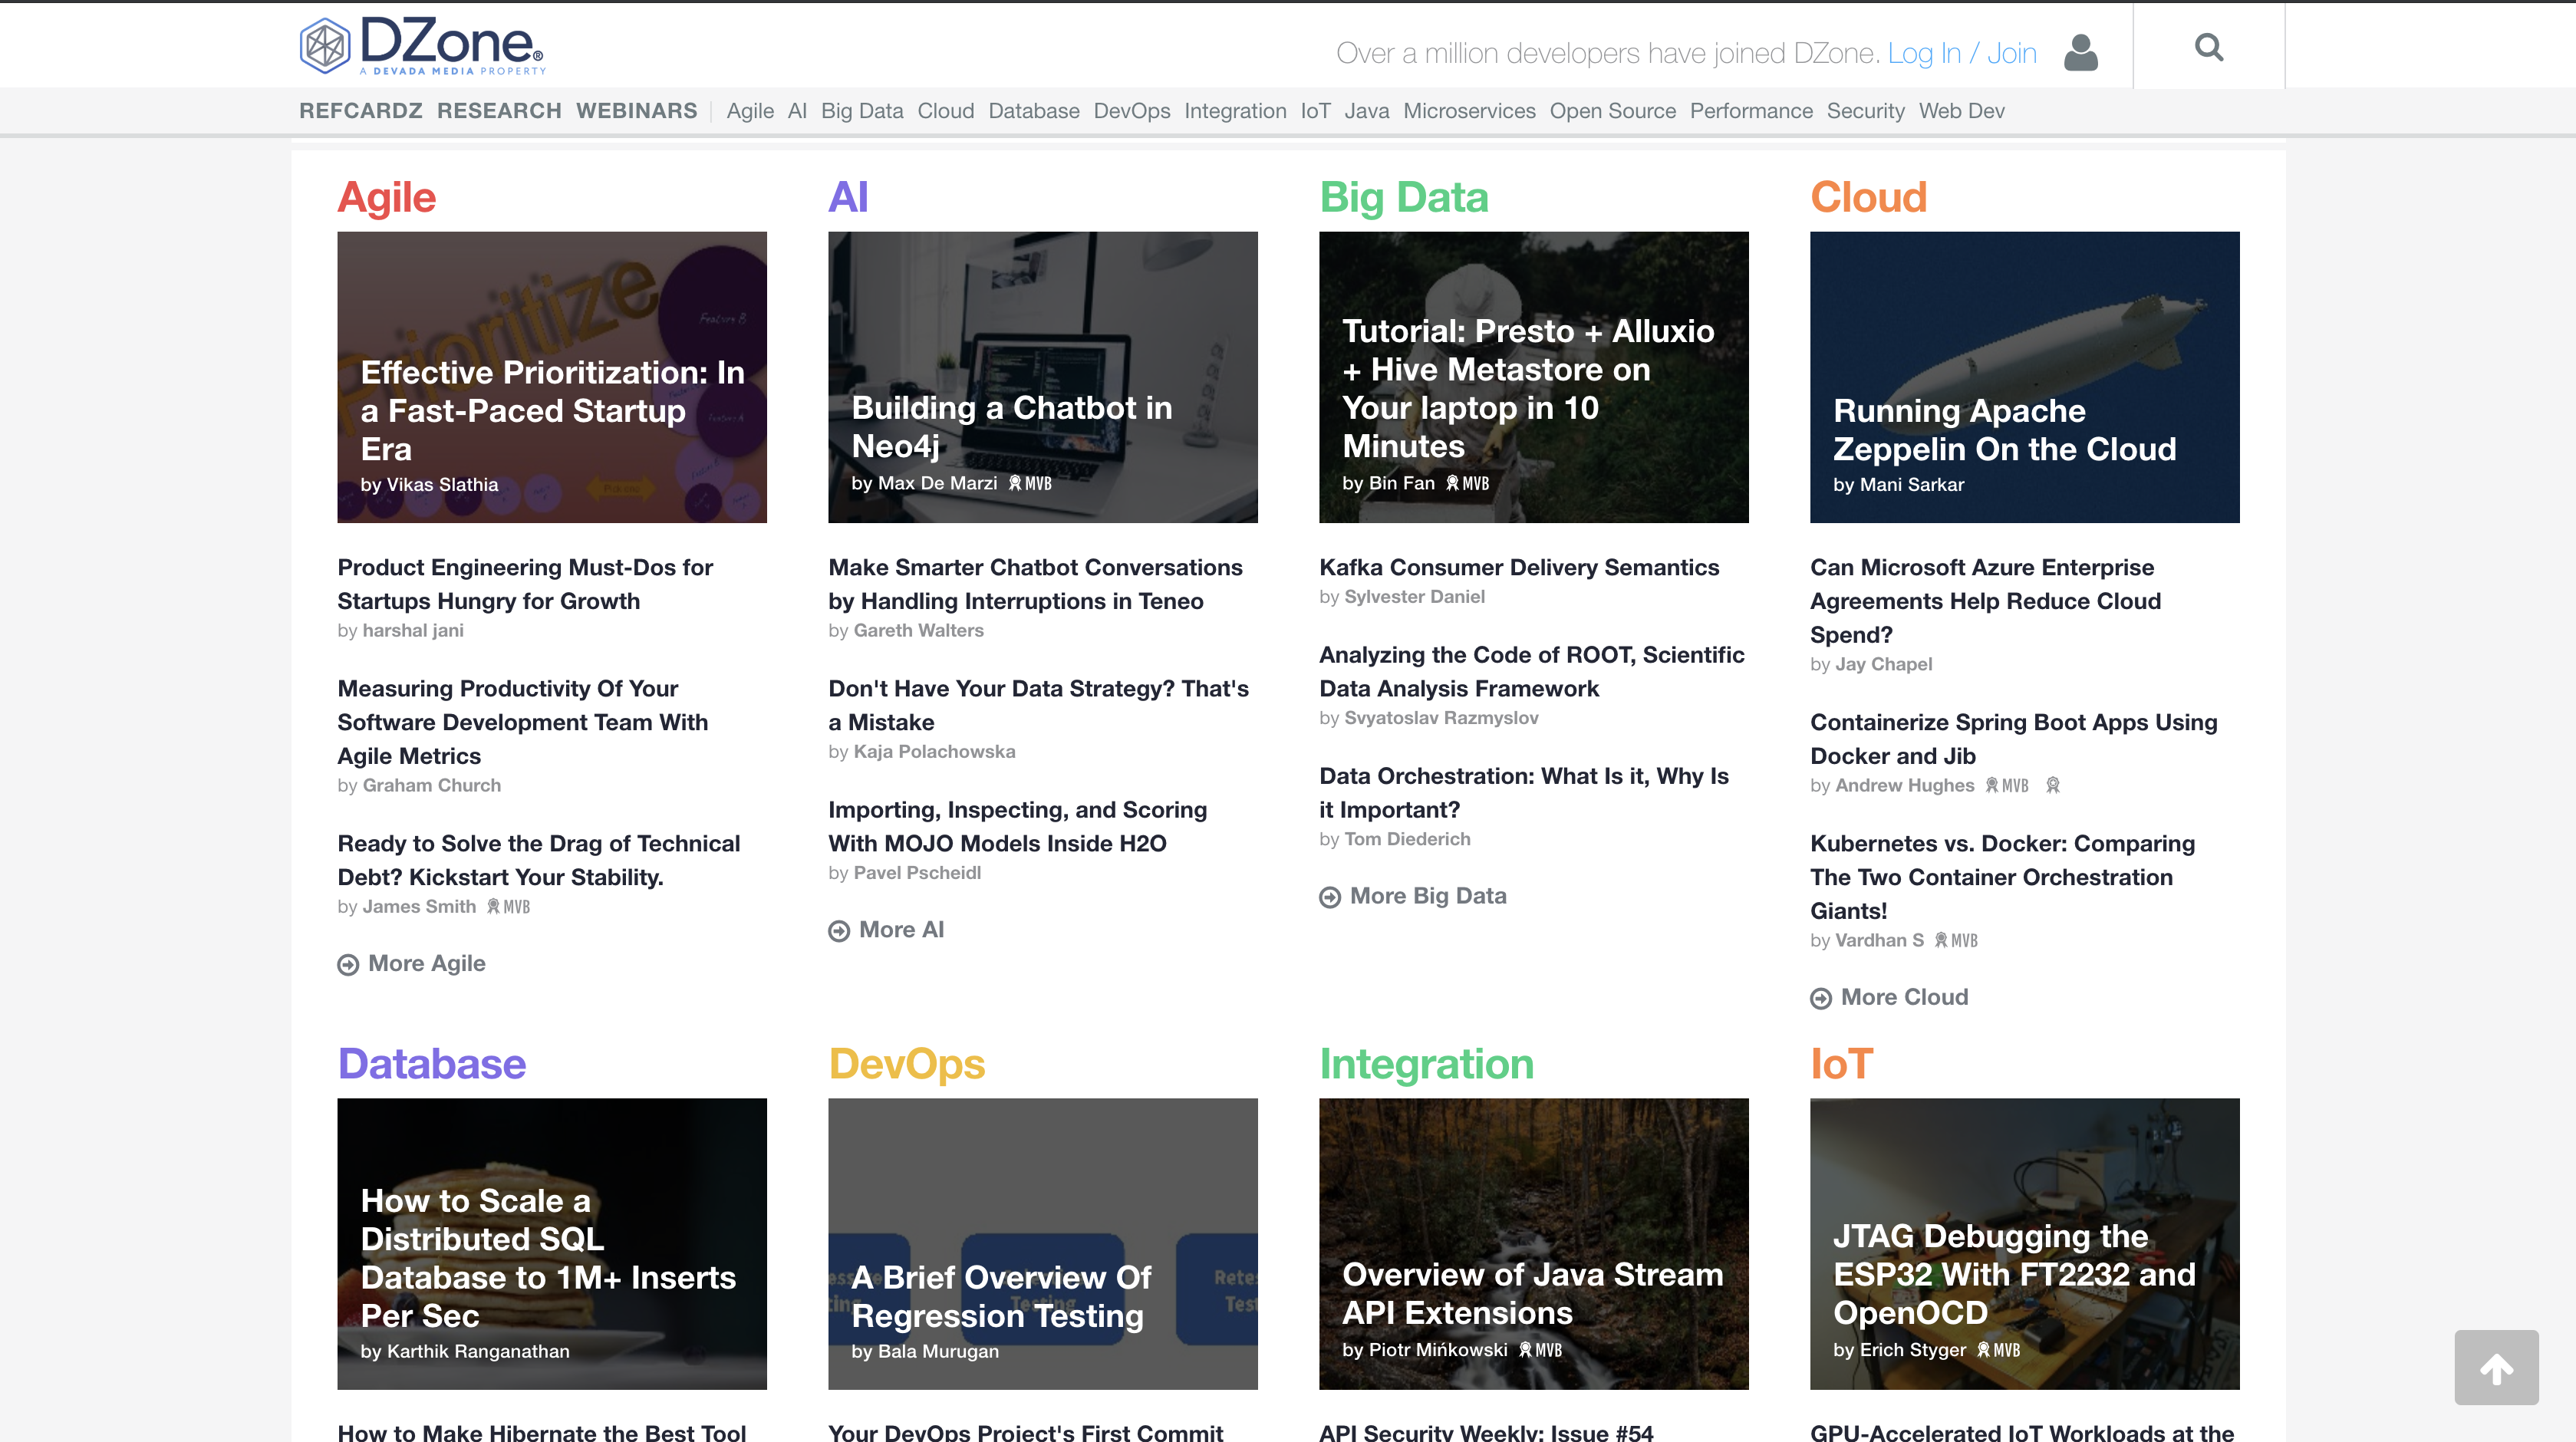
\includegraphics[scale=0.25]{images/DZone}
\end{center}

My application is about a blog system like DZone. It's a web application. It will provide interfaces for some simple operations,
such as querying a article, counting the number of articles for each category, etc. As this project is 
aimed to practise the skills for designing and developing a database but not building a mature product,
my application will only completes very few features of a real blog system and will skip implementing
the querying interfaces for some tables.

For a blog system, we should have some basic entities like User, Article, Comment, Role and Category. User
represents the users of this blog site; Article represents the articles of this blog site; Commtent represents
the comments that users give to some articles; Role represents the role users have, such as administer, common
users; Category represents the article categories, for example, there're categories like Agile, Cloud, DevOps, etc.

Based on these 5 entities, I designed my applications with these 5 interfaces:
\begin{enumerate}
  \item Query users with conditions like username and role. (Select)
  \item Query articles with conditions like username and category (Join)
  \item Add/Update an article (Insert/Update)
  \item Count how many comments each article has (group by \& aggregate)
  \item Delete the articles with the least comments (delete \& subquery)
  \item calculate the average comment amount for articles in each category (group by \& aggregate)
\end{enumerate}









% part 2
\question*{E/R Diagram}

As we discussed in the first section that we have 5 entities, then we can list the attributes for each entity:

For User entity, it will have some attributes: username, nickname, email, description, avatar. Username is the unique id for
this user and it will be used to login; nickname is the name for this user to display on the site and different 
users can use the same nickname; email is the registered email for the user and it is unique; description is a
brief self-description and it could be in 300 letters; avatar is the full URL path of the avatar picture in the 
file system. Username is the primary key.

For Role entity, it will have two attributes: id and roleName. Id is the auto-increment primary key and it has no
specific real meaning; roleName represents the name of this role and it's unique. Id is the primary key.

For Article entity, it will have four attributes: id, title, description and body. Id is the auto-increment primary key and it has no
specific real meaning; title represents the article title; description represents the brief introduction to the article;
body represents the article content. Id is the primary key.

For Comment entity, it will have two attributes: id and content. Id is the auto-increment primary key and it has no
specific real meaning; content represents the comment content. Id is the primary key.

For Category entity, it will have two attributes: id and name. Id is the auto-increment primary key and it has no
specific real meaning; name represents the name of the category. Id is the primary key.

For this blog system, it will also have some relationships:

\begin{enumerate}

\item Users can post new articles. One article will only have a single creater user, but one user can create more thab one 
articles so it's a many-one relationship. 

\item Users can post comments on the article they want to comment as well. It's a multiple relationship. One 
comment can only be posted on one article by one user, but one article can have more than one comments from 
different users. 

\item Each user has a role. One user can only have one role, but one role can be assigned to more than one users.
so it's a many-one relationship. 

\item Each article belongs to a category. One article can belong to more than one categories and one categories 
can have more than one articles. so it's a many-many relationship. 

\end{enumerate}

Based on the above discussion, we can draw a E/R diagram like the following:

\begin{center}
  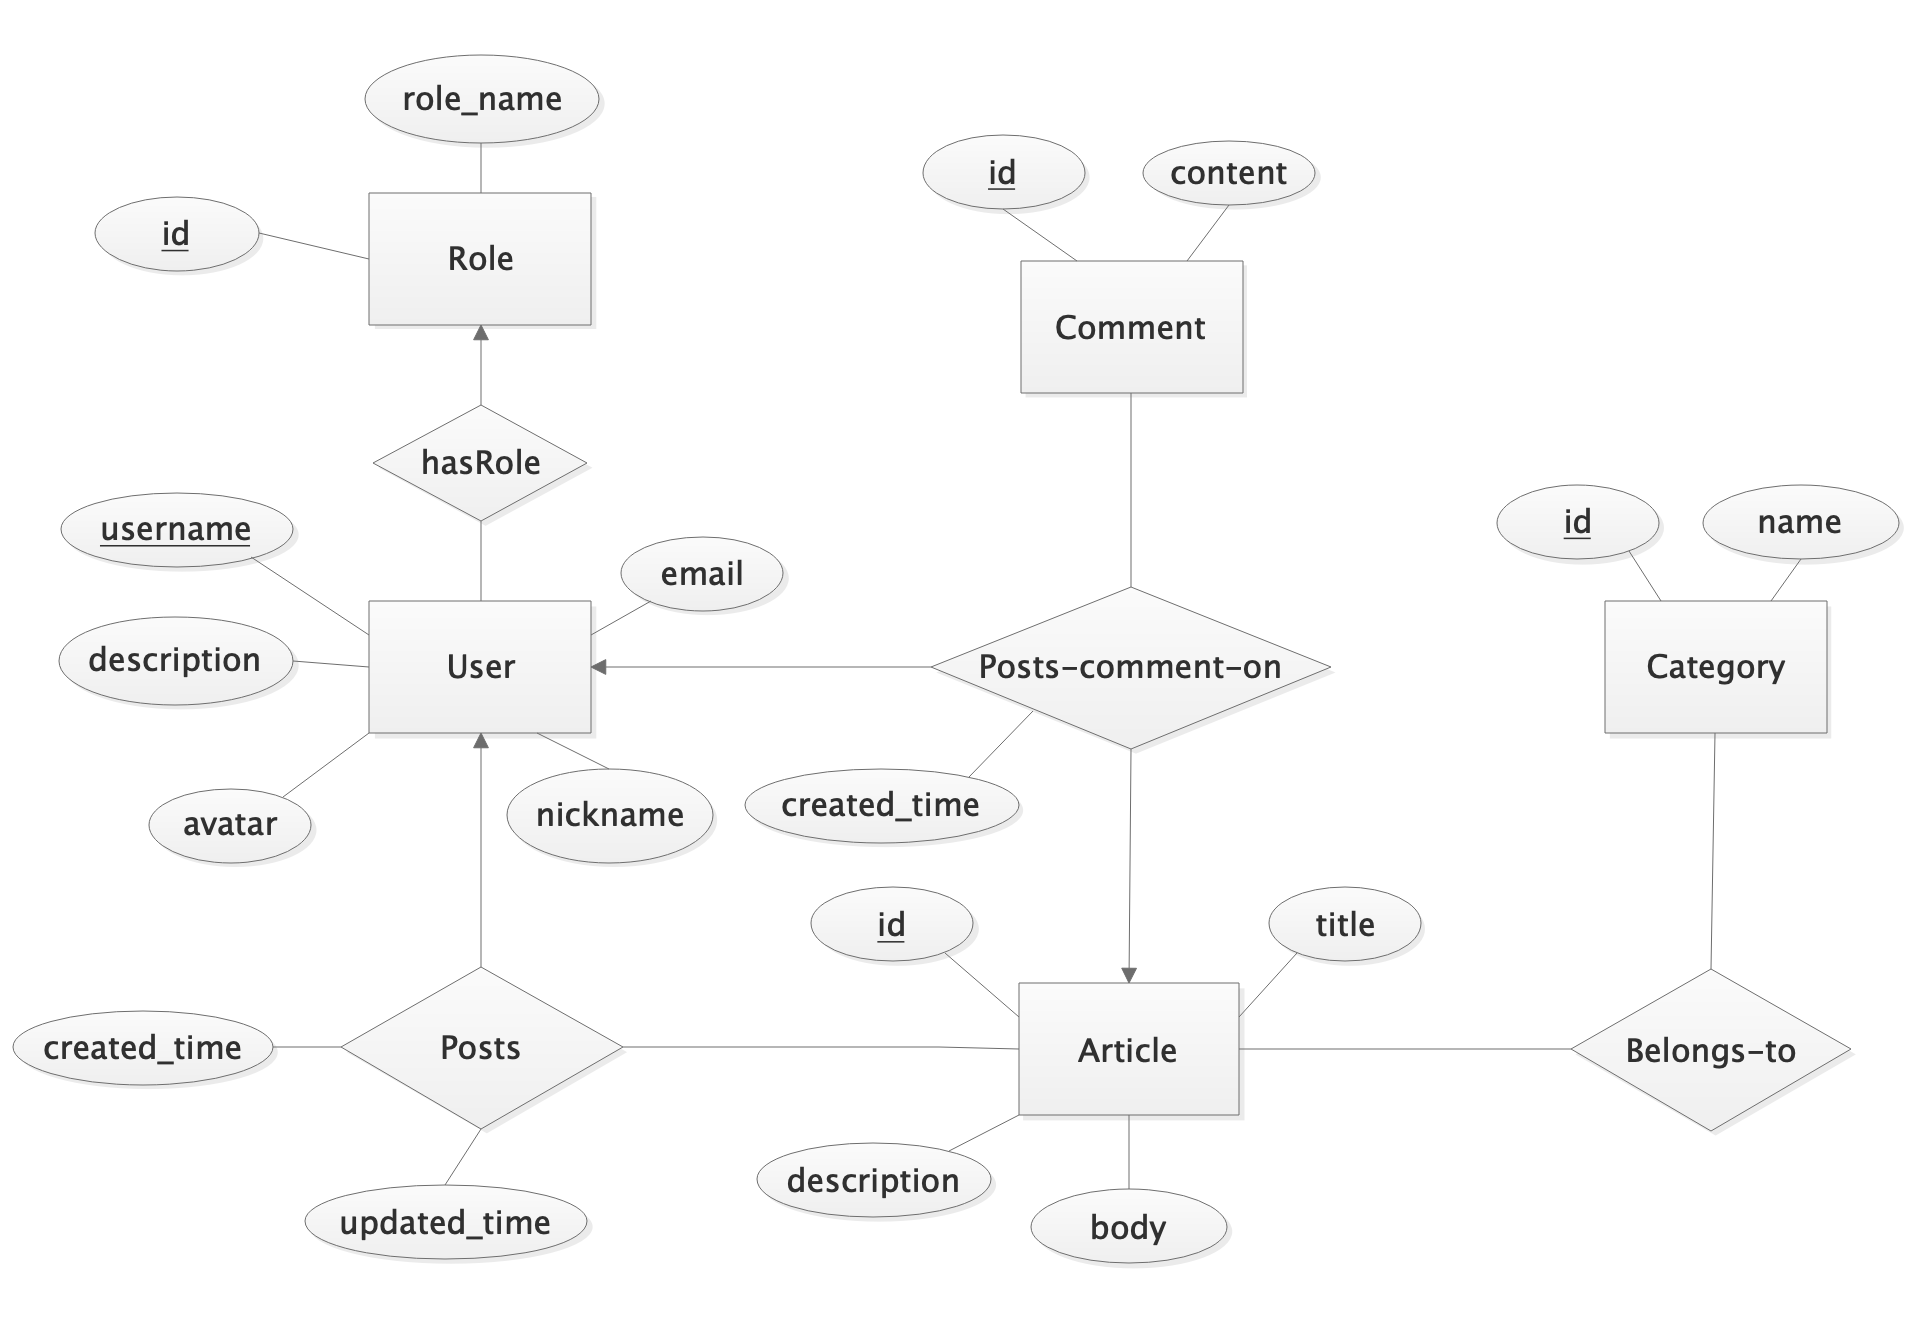
\includegraphics[scale=0.445]{images/ER_Diagram}
\end{center}











% Part 3
\question*{Database Schema and Normalization}

  Transfer the E/R diagram to relations as below:
  \begin{enumerate}
    \item User(\underline{username}, nickname, email, description, avatar)
    \item Role(\underline{id}, roleName)
    \item hasRole(\underline{username}, \underline{roleId})
    \item Article(\underline{articleId}, title, description, articleBody)
    \item Posts(\underline{username}, \underline{articleId}, createdTime, updatedTime)
    \item Comment(\underline{commentId}, commentContent)
    \item PostsCommentOn(\underline{username}, \underline{commentId}, \underline{articleId}, createdTime)
    \item Category(\underline{categoryId}, categoryName)
    \item BelongsTo(\underline{articleId}, \underline{categoryId})
  \end{enumerate}

  The nontrivial FDs in each relation:
  \begin{enumerate}
    \item User's FDs: \{username $\rightarrow$ \{nickname, email, description, avatar\}, email $\rightarrow$ username\}
    \item Role's FDs: \{roleId $\rightarrow$ roleName\}
    \item hasRole's FDs: $\emptyset$
    \item Article's FDs: \{articleId $\rightarrow$ \{title, description, articleBody\}\}
    \item Posts's FDs: \{\{username, articleId\} $\rightarrow$ \{createdTime, updatedTime\}\}
    \item Comment's FDs: \{commentId $\rightarrow$ commentContent\}
    \item PostsCommentOn's FDs: \{\{username, commentId, articleId\} $\rightarrow$ createdTime\}
    \item Category's FDs: \{categoryId $\rightarrow$ categoryName\}
    \item BelongsTo's FDs: $\emptyset$
  \end{enumerate}

  Then we check whether each relation is in BCNF:
  \begin{enumerate}
    \item For User: username and email are two candidate keys. The left sides are all superkeys. Therefore, User is in BCNF.
    \item For Role: roleId is the only key. The left sides are all superkeys. Therefore, Role is in BCNF.
    \item For hasRole: As the FDs is an empty set, BelongsTo is in BCNF.
    \item For Article: articleId is the only key. The left sides are all superkeys. Therefore, Article is in BCNF.
    \item For Posts: \{username, articleId\} is the only key. The left sides are all superkeys. Therefore, Posts is in BCNF.
    \item For Comment: commentId is the only key. The left sides are all superkeys. Therefore, Comment is in BCNF.
    \item For PostsCommentOn: \{username, commentId, articleId\} is the only key. The left sides are all superkeys. Therefore, PostsCommentOn is in BCNF.
    \item For Category: articleId is the only key. The left sides are all superkeys. Therefore, Category is in BCNF.
    \item For BelongsTo: As the FDs is an empty set, BelongsTo is in BCNF.
  \end{enumerate}

  Therefore, we can conclude these relations are all in BCNF.

  Since we have some many-one relationships, we can try to merge them to the "many" side of entity. After merging, we can get
  a set of new relations:
  \begin{enumerate}
    \item User(\underline{username}, nickname, email, description, avatar, roleId)
    \item Role(\underline{roleId}, roleName)
    \item Article(\underline{articleId}, \underline{username}, title, description, articleBody, createdTime, updatedTime)
    \item Comment(\underline{commentId}, \underline{username}, \underline{articleId}, commentContent, createdTime)
    \item Category(\underline{categoryId}, categoryName)
    \item BelongsTo(\underline{articleId}, \underline{categoryId})
  \end{enumerate}
  
  The nontrivial FDs in this new relation set:
  \begin{enumerate}
    \item User's FDs: \{username $\rightarrow$ \{nickname, email, description, avatar, roleId\}, email $\rightarrow$ username\}
    \item Role's FDs: \{roleId $\rightarrow$ roleName\}
    \item Article's FDs: \{articleId $\rightarrow$ \{username, title, description, articleBody\}, \{username, articleId\} $\rightarrow$ \{createdTime, updatedTime\}\}
    \item Comment's FDs: \{commentId $\rightarrow$ username, articleId, commentContent, \{username, commentId, articleId\} $\rightarrow$ createdTime\}
    \item Category's FDs: \{categoryId $\rightarrow$ categoryName\}
    \item BelongsTo's FDs: $\emptyset$
  \end{enumerate}

  Definitely, there're some changes in these two relations: Article and Comment.

  \begin{enumerate}
    \item For User, the only key is username. So User is in BCNF.
    \item For Article, the only key is articleId. So Article is in BCNF.
    \item For Comment, the only key is commentId. So Comment is in BCNF.
  \end{enumerate}

  Therefore, we can conclude these modified relations are still all in BCNF.

  % TODO
  I think it's hard to improve my schemas by 3NF and 4NF, because the FDs of current schemas are mostly in the pattern
  that primary key determines the other attributes. 



















% Part 4
\question*{Creating Tables}
  Based the analysis in the above sections, We can design the SQL schemas like the following:

  \newpage

  \begin{table}[h!]
    \begin{center}
      \caption{User}
      \label{tab:table1}
      \begin{tabular}{c|c|c} % <-- Alignments: 1st column left, 2nd middle and 3rd right, with vertical lines in between
        \textbf{Attribute Name} & \textbf{Datatype} & \textbf{Comment}\\
        \hline
        id & INT & primary key; not null; auto increment \\
        username & VARCHAR(45) & unique; not null \\
        nickname & VARCHAR(45) & not null \\
        email & VARCHAR(256) & unique; not null \\
        description & VARCHAR(300) & a brief personal description; it could be null \\
        avatar & VARCHAR(45) & a URL refered to the avatar picture; it could be null \\
      \end{tabular}
    \end{center}
  \end{table}

  \begin{table}[h!]
    \begin{center}
      \caption{Role}
      \label{tab:table4}
      \begin{tabular}{c|c|c} % <-- Alignments: 1st column left, 2nd middle and 3rd right, with vertical lines in between
        \textbf{Attribute Name} & \textbf{Datatype} & \textbf{Comment}\\
        \hline
        id & INT & primary key; not null; auto increment \\
        name & VARCHAR(45) & role name; not null; unique \\
      \end{tabular}
    \end{center}
  \end{table}

  \begin{table}[h!]
    \begin{center}
      \caption{Article}
      \label{tab:table2}
      \begin{tabular}{c|c|c} 
        \textbf{Attribute Name} & \textbf{Datatype} & \textbf{Comment}\\
        \hline
        id & BIGINT & primary key; not null; auto increment \\
        username & VARCHAR(45) & foreign key to table User; not null \\
        title & VARCHAR(100) & article title; not null \\
        description & VARCHAR(500) & brief description; not null \\
        body & BLOB & article body; it could be very large; not null \\
        created\_time & TIMESTAMP & using current timestamp as default value \\
        updated\_time & TIMESTAMP & it will be set to the current timestamp on update \\
      \end{tabular}
    \end{center}
  \end{table}

  \begin{table}[h!]
    \begin{center}
      \caption{Comment}
      \label{tab:table3}
      \begin{tabular}{c|c|c} % <-- Alignments: 1st column left, 2nd middle and 3rd right, with vertical lines in between
        \textbf{Attribute Name} & \textbf{Datatype} & \textbf{Comment}\\
        \hline
        id & BIGINT & primary key; not null; auto increment \\
        username & VARCHAR(45) & foreign key to table User; not null \\
        article\_id & BIGINT & foreign key to table Article; not null \\
        content & VARCHAR(1024) & comment content; not null \\
        created\_time & TIMESTAMP & using current timestamp as default value \\
      \end{tabular}
    \end{center}
  \end{table}

  \begin{table}[h!]
    \begin{center}
      \caption{Category}
      \label{tab:table4}
      \begin{tabular}{c|c|c} % <-- Alignments: 1st column left, 2nd middle and 3rd right, with vertical lines in between
        \textbf{Attribute Name} & \textbf{Datatype} & \textbf{Comment}\\
        \hline
        id & INT & primary key; not null; auto increment \\
        name & VARCHAR(80) & category name; not null; unique \\
      \end{tabular}
    \end{center}
  \end{table}

  \begin{table}[h!]
    \begin{center}
      \caption{Belongs To}
      \label{tab:table5}
      \begin{tabular}{c|c|c} % <-- Alignments: 1st column left, 2nd middle and 3rd right, with vertical lines in between
        \textbf{Attribute Name} & \textbf{Datatype} & \textbf{Comment}\\
        \hline
        id & INT & primary key; not null; auto increment \\
        article\_id & BIGINT & foreign key to table Article; not null \\
        category\_id & INT & foreign key to table Category; not null \\
      \end{tabular}
    \end{center}
  \end{table}

  \newpage

  The SQL DDL script is in the source file, please see more information in README.


















\question*{Data generation}

  I choose to get my data by generating some fabricate data.

  First, I use random strings with different length to fill the usename, nickname, email, 
  description, avatar attributes for a user.

  Then, for each user I simulated the process of creating 10 articles. I also use random strings with
  different length to fill the attributes for an article.
  
  Also, for each user I simulated the process of creating 10 comments. But I will fill the attribute of
  articleId as 1 initially. Because the comments should be pointed to one article and we can't assigned the 
  articleId before we generating all articles. After we generate all the articles, we can re-scan the 
  comments csv and generate the articleId again.

  For Category and Role, they are all small tables. So we can generate the data before we start to generate
  User, Article and Comment.

  For more explanation, please see the README file.















% Question 5
\question*{User Interface and Functions}

I use Vue.js to build the frontend pages and use Java and Spring Framework to build the backend service.

For more explanation, please see the README file.







\end{document}
